% 使用 Beamer 类来创建演示文稿
\documentclass{beamer}

% 使用 ctexcap 宏包来支持中文,UTF8 编码,无缩进
\usepackage[UTF8,noindent]{ctexcap}

% 使用 tikz 宏包来绘图
\usepackage{tikz}

% 使用 graphicx 宏包来插入图片
\usepackage{graphicx}

\usepackage{romannum}

% 选择 Berlin 主题
\usetheme{Berlin}

% \usecolortheme{crane} % 可以选择一个颜色主题,但这里被注释掉了

% 设置机构名称及其缩写
\institute[NJUPT]{南京邮电大学}

% 设置作者及其缩写
\author[Robert$\cdot$Charlie]{贺昌嘉}

% 设置文档标题及其缩写
\title[学期总结]{学期总结}

% 设置文档日期为今天
\date{\today}

% 设置文档副标题
\subtitle{这是文档的小标题}

% 设置文档主题
\subject{总结PPT}

% 设置背景图位置,这里的 xshift 和 yshift 可以调节相对位置
%\titlegraphic{
\includegraphics[width=0.5\textwidth]{beamer图片1.png}}

% 设置 logo 模板,在左上角插入校徽图片
\setbeamertemplate{logo}{%
	\begin{tikzpicture}[overlay, remember picture]
		\node[xshift=15em,yshift=-13em] at (current page.north west) {
\includegraphics[height=.1\paperheight]{校徽.jpg}};
		%\node[xshift=-8.13em,yshift=-1.8em,opacity=.3] at (current page.east) {
\includegraphics[height=.7\paperheight]{NJUPT.png}};
		\node[xshift=-20.86em,yshift=-9.5em,opacity=.3] at (current page.east) {
\includegraphics[scale=0.5]{NJUPT.png}};
	\end{tikzpicture}
}

% 开始文档内容
\begin{document}
	
	% 生成标题页
    \begin{frame}
    	\maketitle
    \end{frame}
	
	% 重置 logo 模板
	\setbeamertemplate{logo}{} 
	
	% 设置背景模板,在右侧插入 NJUPT.png 图片并设置透明度
	\setbeamertemplate{background}{
		\begin{tikzpicture}[overlay, remember picture]
			\node[xshift=-8.13em,yshift=-1.8em,opacity=.3] at (current page.east) {
\includegraphics[height=.7\paperheight]{NJUPT.png}};
		\end{tikzpicture}
	}
	
	% 创建目录页
	\begin{frame}{目录}
		\tableofcontents
	\end{frame}
	
	% 第一部分
	\section{折腾的一学期}
	
	% 创建一个幻灯片,设置标题和小标题
	\begin{frame}{在折腾中}{发现新世界}
		\begin{itemize}
		\visible<1->{	\item[1] 学期刚开始的时候学习 \LaTeX , 大概一个半月的时间都在折腾. 
			}
		\visible<2->{	\item[2] 买了一台新的平板,开始折腾平板上应用
			}
		\visible<3->{	\item[3] 折腾电子资料(总喜欢收集电子资料)
	}
		\visible<4->{	\item[4] 折腾软件:捣鼓一些稀奇古怪的软件,虽然事后也没怎么用过.
	}
		\end{itemize}
	\end{frame}
	
	% 第二部分
	\section{收获的一学期}
	
	% 创建一个幻灯片,设置标题和小标题
	\begin{frame}
		\frametitle{在行中知}
		\framesubtitle{技术收获满满}
		\begin{itemize}[<+->]
			\item[A] 成功拿下一次奖学金
			\item[B] 和好朋友跑了人生第一场马拉松
			\item[C] 学习了\LaTeX,Markdown等语法
			\item[D] 成功申请到了Github-Education
			\item[E] 学会使用git,github等版本控制软件,还需要进一步提升.
		\end{itemize}
	\end{frame}
	
	% 第三部分
	\section{遗憾的一学期}
	
	% 创建一个幻灯片,包含项目列表
	\begin{frame}
		\frametitle{略带遗憾}
		\framesubtitle{等待2025的自己去弥补}
		\begin{itemize}[<+->]
			\item[a] 还没有谈一场甜甜的恋爱 
			\item[b] 专业课没有花相应的时间去学习拓展
			\item[c] 体育,体育课成绩和体测成绩都下滑的很厉害
			\item[d] 没有系统性的去学习某一知识.
			\item[e]  理论知识增长很少
			\item[f] 数学竞赛没有准备充分,只拿了个参水的三等奖.
 		\end{itemize}
	\end{frame}
	
	% 第四部分
	\section{对下学期的展望}
	
	% 创建一个幻灯片,包含有序列表和引用部分
	\begin{frame}
		\frametitle{有所期待}
		\framesubtitle{Why not try your best!!!}
		\begin{enumerate}[<+->]
			\item[\Romannum{1}] 找好自己该走的路,反正照现在这情况来看,肯定是去考研了
			\item[\Romannum{2}] 谈次恋爱,\small{谈不到就算了}
			\item[\Romannum{3}]学好理论知识,数学,算法,编程
			\item[\Romannum{4}]进一步熟悉自己的工作流,熟悉,精通几款软件.
%			% 引用部分
%			这是引用部分:
%			\begin{quote}
%				\item[a] Hope You Like It.
%				\item[b] Have a Good Day!
%			\end{quote}
		\end{enumerate}
	\end{frame}
	
%	% 第五部分
	\section{综上所述}
%	
%	% 创建一个幻灯片,设置标题和小标题
	\begin{frame}
		\frametitle{静水流深}
		\framesubtitle{我还年轻,路还正长,不设限制}
		向干啥就去干吧,别等以后没有机会空留遗憾
		
		现在比较有感触的两句诗:
		\begin{block}{《锦瑟》-李商隐}
			此情可待成追忆,只是当时已惘然。
		\end{block}
		\begin{block}{《过松源晨炊漆公店》-杨万里}
			正入万山围子里,一山放过一山拦
		\end{block}
	\end{frame}
	\begin{frame}
		\only<1>{
\includegraphics[width=\paperwidth,height=\paperheight,keepaspectratio]{1.png}}
		\only<2>{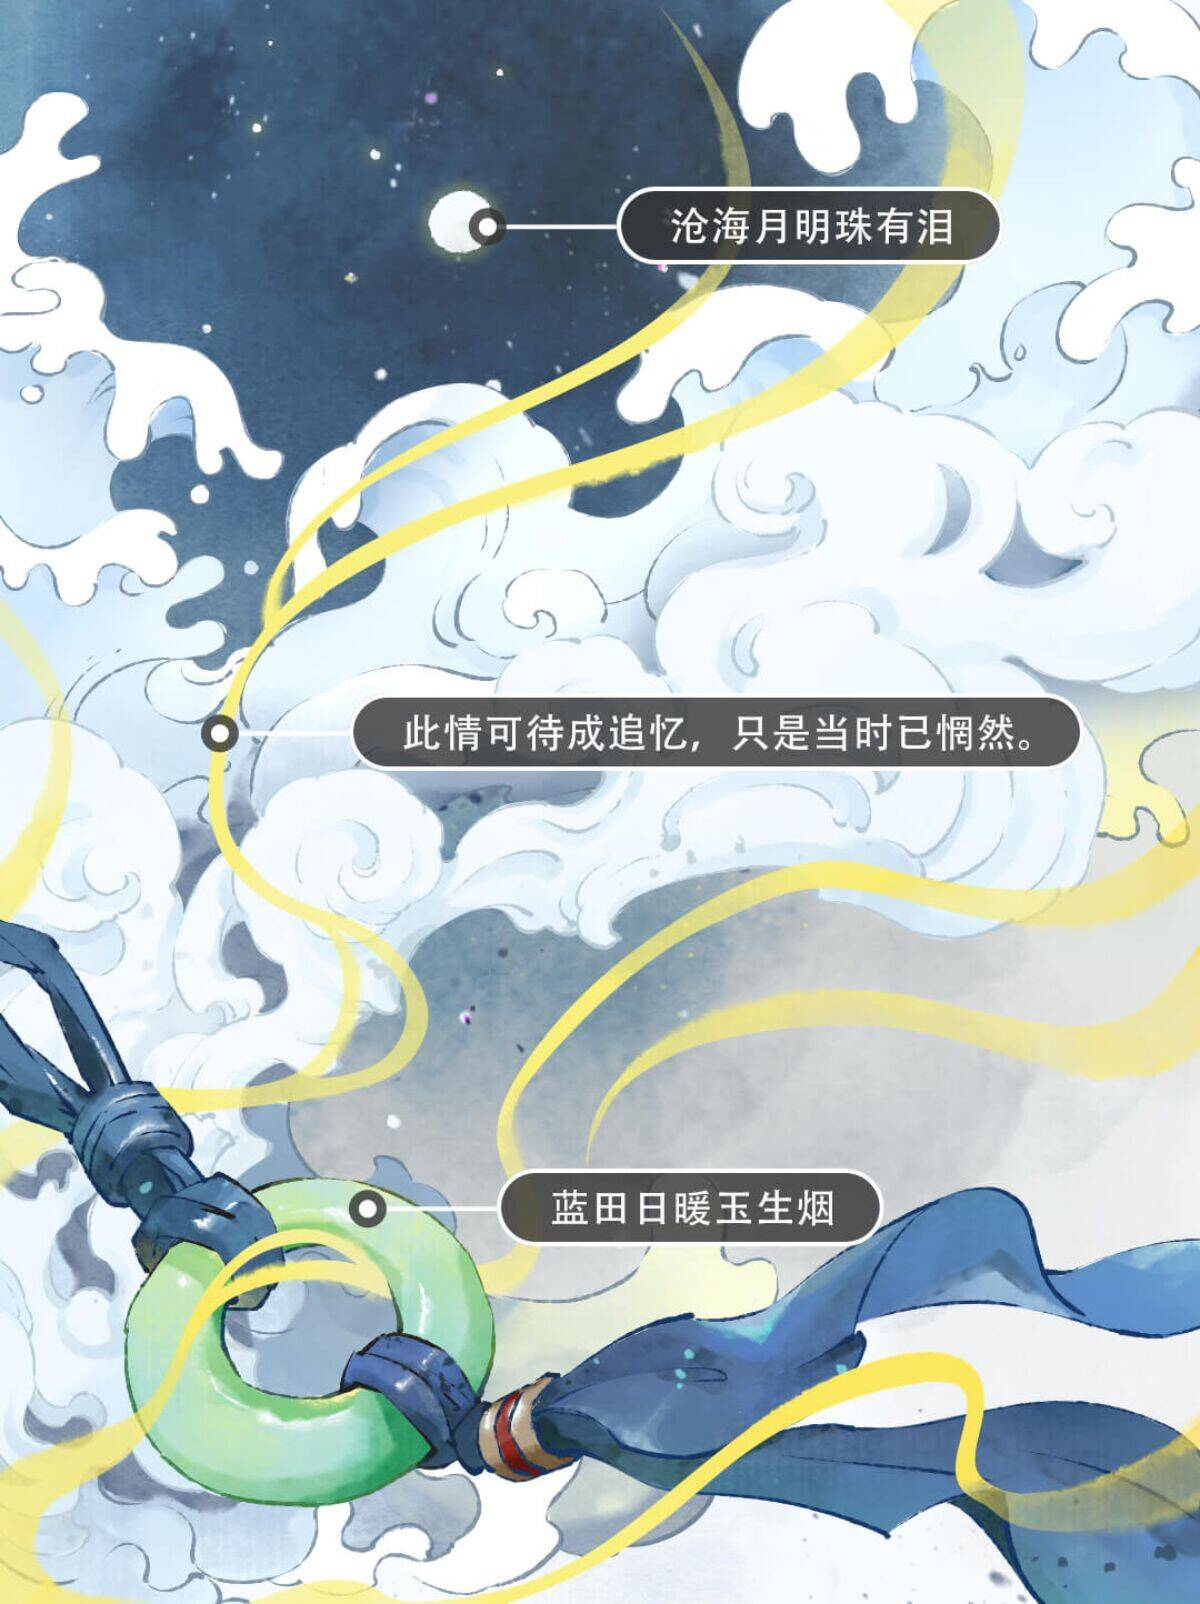
\includegraphics[width=\paperwidth,height=\paperheight,keepaspectratio]{2.png}}
		\only<3>{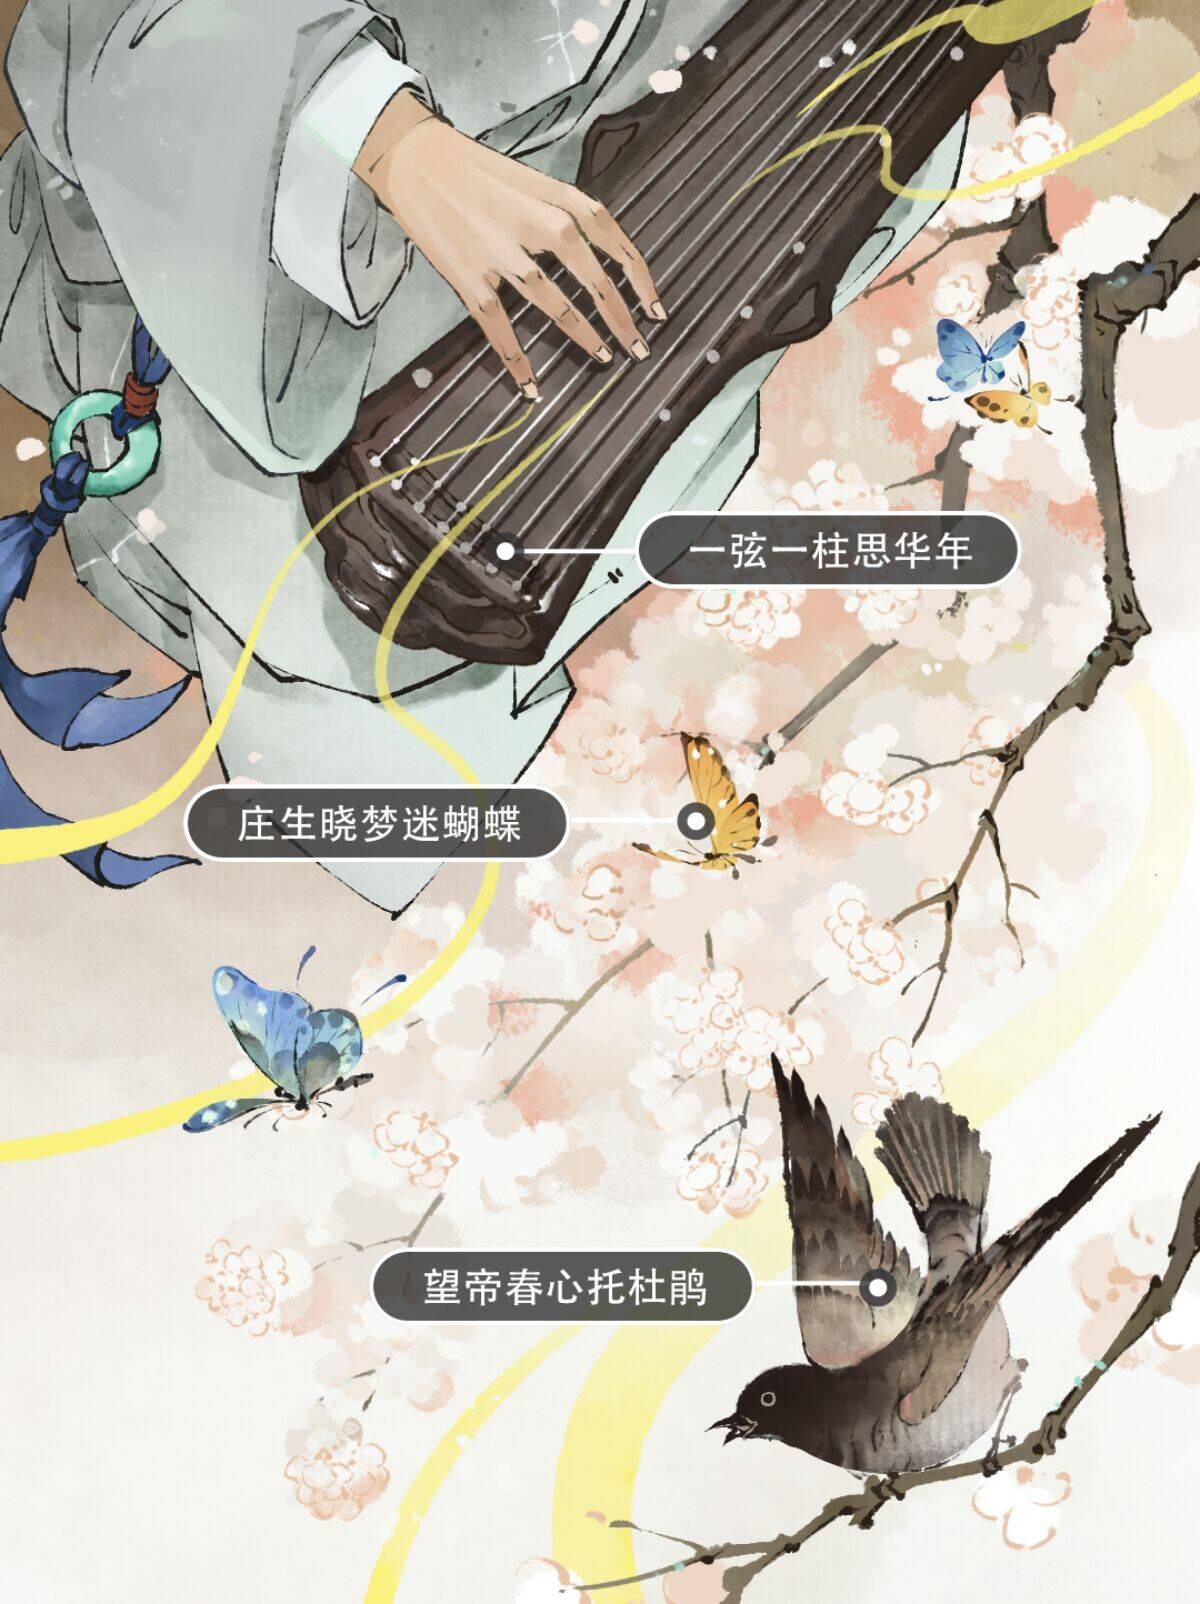
\includegraphics[width=\paperwidth,height=\paperheight,keepaspectratio]{3.png}}
		\only<4>{
\includegraphics[width=\paperwidth,height=\paperheight,keepaspectratio]{4.png}}
	\end{frame}
	
	\begin{frame}{结语}
		
		谢谢大家耐心的观看!
	\end{frame}
	% 结束文档
\end{document}